%
%
%
\section{Ordinary least squares (OLS)}

	%
	% 5.2.1
	%
	\subsection{Empirical introduction}

Our research question in this chapter uses the \QOG{} dataset to examine how education if and how religion and education compete over the issue of abortion. The dataset provides country-level information, at which we can observe population-level factors and system-level effects derived from political or social institutions.

The level of support for abortion in the population will be our dependent variable, measured as the average answer to the question ``Please tell me whether you think abortion can always be justified, never be justified, or something in between'' asked in the \WVS{} between 1996 and 2008. At the individual level, the answers ranged from (1) ``Never justifiable'' to (10) ``Always justifiable.''

Figure~\ref{fig:distr} shows the distribution of the measure over selected regions of the world for which there are a sufficient number of observations to detect outliers. A series of $t$-tests would show that European populations express significantly higher levels of support for abortion than African populations. In the overall \QOG{} data, the variable \texttt{wvs\_abort} holds the aggregate mean of answers for $N = 94$ countries. 

In the two regional clusters outlined above, Israel markedly differs from African and Middle Eastern countries by its higher support for abortion. The exceptionality of Israel might be a useful heuristic if one considers some salient characteristics of Israeli society, such as higher levels of education and high levels of gender equality. Israel is actually much closer to European countries than it is to African and Middle Eastern ones when compared on measures of gender equality or gender gaps.\footnote{\label{fn:gdi_gem} The United Nations Development Programme, the World Bank and the World Economic Forum all produce indices that serve this comparison. See variables \texttt{undp\_gdi undp\_gem wdi\_gris wef\_gend} in the \QOG{} dataset.}

\begin{figure}[htp]
	\centering
	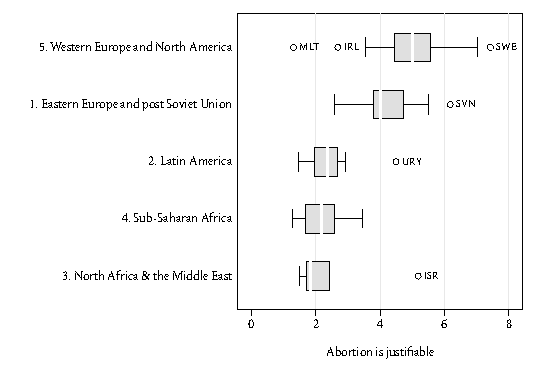
\includegraphics[width=.9\textwidth]{images/abortion_box.pdf}

	\caption[Regional distributions of support for abortion]{\label{fig:distr}
	Selected regional distributions of support for abortion. %
  \qog}
	
\end{figure}%

\begin{docspec}
	* graph code: plot regional subsets\\%
	gr hbox wvs\_abort if ht\_region2 < 6, ///\\%
	  over(ht\_region2, sort(1)des) mark(1, mlab(ccodewb))
\end{docspec}

Our explanatory intuitions so far lie with the presumed effect of education systems and gender equality on support for abortion, which is also observable in Asian and Latin American countries. However, religious authorities, which we assume to be opposed to abortion at least in principle, can be either providers or strong moral sources of education. The data contain measures of religiousness and religiosity that can be used next to education in order to determine how much of a zero-sum game these factors play with each other.

Finally, we will take into account the expected effect of democratic politics over the issue by separating democracies and dictatorships. We therefore start this chapter with a composite explanatory model that covers religion, education, gender and political institutions. Our intention is to derive a model that allows to measure the \emph{independent}, net effect of each variable onto the aggregate level of support for abortion in each country. Additional controls will be introduced for wealth, measured as gross domestic product per capita, and fertility rates.

	%
	% 5.2.2
	%
  \subsection{Visualizing a linear model}%
  	\index{Models|see{Linear regression}}%
  	\index{Linear regression!Linear models}

Figures~\ref{fig:model_quadrant_top} and~\ref{fig:model_quadrant_bottom} show how a simple linear model links the dependent variable $Y$ (support for abortion) to an independent variable $X$ mass education, measured as the average years of schooling in the population aged 25 and above.\footnote{The data come from the \href{http://www.hks.harvard.edu/centers/cid}{Center for International Development at Harvard University}, where it was rounded up by Robert J. Barro and Jong-Wha Lee.} The next sections will explain each graph in detail and cover each step of their analysis.

\paragraph{Variance} The left graph shows the dispersion of $Y$ and $X$ around their respective means, and the right graph shows how the model makes sense of it: the variance of $X$ (in blue) will be used to predict the variance of $Y$ (in red), using a linear estimator of the form $Y = f(X) + \epsilon$.

\begin{figure}[htp]
	\centering
	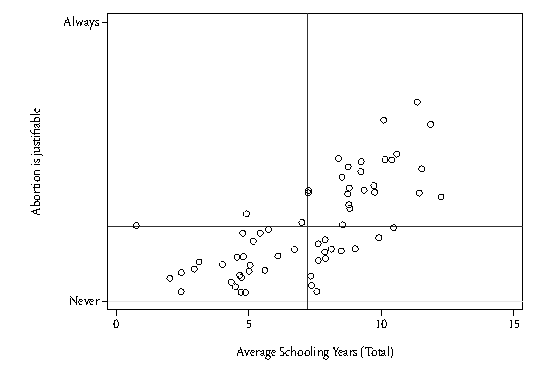
\includegraphics[width=.6\textwidth]{images/abortion_sc_means.pdf}\\
	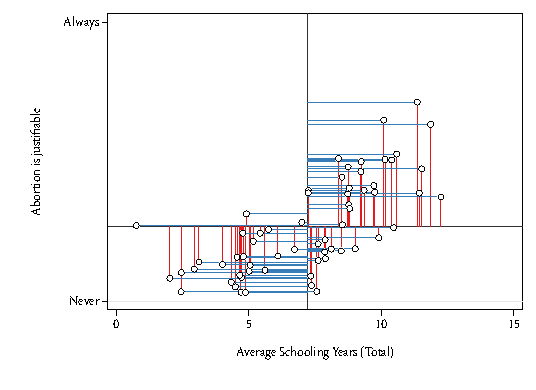
\includegraphics[width=.6\textwidth]{images/abortion_sc_variance.pdf}

	\caption[Support for abortion and mass education (1): Variance]{\label{fig:model_quadrant_top}%
	Scatterplots of variance in support for abortion and mass education. %
	\qog}
\end{figure}%

\paragraph{Model} The top graph shows the linear fit of a simple linear regression, which is the straight line representing the linear function $Y = \alpha + \beta X$, on which each data point has a predicted--or fitted--equivalent. The bottom graph shows how much of the variance of $Y$ it successfully predicts (in green), and how much of it is left unpredicted, or unexplained, by the linear regression model (in red).

\begin{figure}[htp]
	\centering
	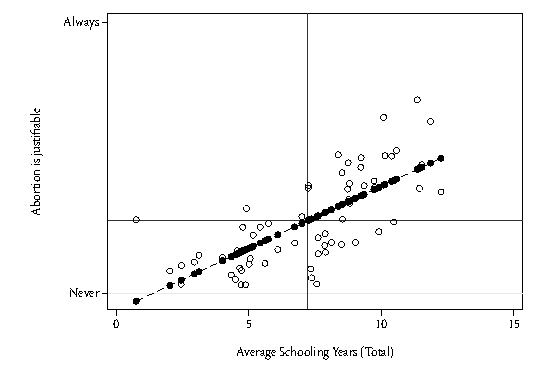
\includegraphics[width=.6\textwidth]{images/abortion_sc_lfit.pdf}\\
	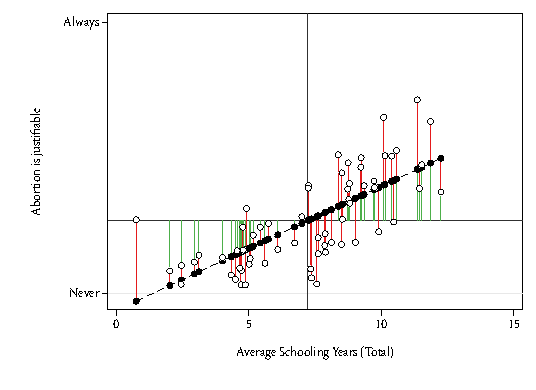
\includegraphics[width=.6\textwidth]{images/abortion_sc_gfit.pdf}

	\caption[Support for abortion and mass education (2): Model]{\label{fig:model_quadrant_bottom}%
	Scatterplots of a linear model predicting support for abortion from mass education. %
	\qog}
\end{figure}%

The very last graph that we drew for this model indicates that the linear estimator is predicting roughly half of the variance in $Y$ from the variance of $X$. Furthermore, the variance predicted by the model is distributed evenly over the data, which means that the linear estimator is performing efficiently in the overall data, and not just in selected areas. The unpredicted variance of the model will be analyzed after we explain how the estimator works in practice.

	%
	% 5.2.3
	%
	\subsection{Linear fitting}

  The relationship between two or more variables can be represented by a \emph{linear fit} of the data. In statistical terms, this result can be obtained by minimizing the \emph{residual sum of squares} (RSS), \ie the fraction of the variance $\epsilon$ left unexplained by a linear estimator $Y = \alpha + \beta X + \epsilon$, where $Y$ and $X$ are respectively the dependent and independent variable(s), a.k.a the \emph{predictors}.

  To explain how this works, we will use Douglas Hibbs' `Bread and Peace' voting model for the U.S. presidential election, which was recently updated to assess Barack Obama re-election prospects.\cite{Hibbs:2012a} The model understands the election votes as a function of the economy, measured in effective variation of wealth at the individual level. Under some historical circumstances, the number of deaths in the U.S. military is added as a significant factor. The compound effect of these factors is called `bread and peace' voting and is a form of retrospective voting theory.

  Figure~\ref{fig:hibbs_data} shows how the `voting' and `bread' variables are distributed. Their association shows a strong, positive linear relationship ($\text{Pearson's}~\rho \approx .8$).

  \begin{figure}[htp]
  	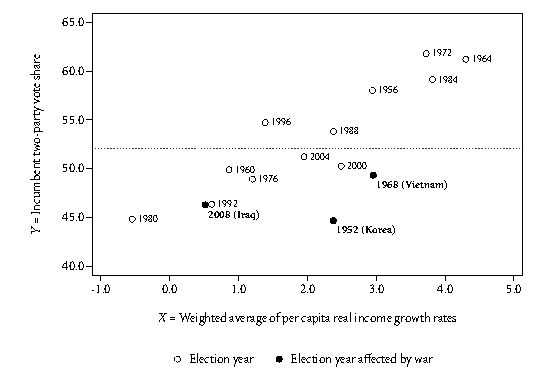
\includegraphics[width=.9\textwidth]{images/hibbs1.pdf}

  	\caption[U.S. presidential elections]{\label{fig:hibbs_data}
  	U.S. presidential elections and the economy, 1952--2008. %
  	Line at mean value $\bar Y$ (dependent variable). %
    \hibbs}
  \end{figure}%

  Figure~\ref{fig:hibbs_fit} shows what a linear estimator of the form $Y = \alpha + \beta X + \epsilon$ does in practice. The mean value of the dependent variable corresponds to a `null estimator' where the effect (or influence) of $X$ on $Y$ is null, \ie $\beta = 0$ and $Y = \alpha$, which defines a constant function shown as a vertical line. The line that reduces as much as possible the squared deviations between its points and the data is called the \emph{regression line}, or a \emph{linear fit}. Each data point has a corresponding point on that line, called the \emph{fitted value}. The variance that is better predicted by this model than by a null estimator is shown in green, while the residuals of the model, \ie the fraction of variance unexplained by its variables, are shown in red.\footnote{The graphs should have reminded you of Figure~\ref{fig:model_quadrant_bottom} at p.~\pageref{fig:model_quadrant_bottom}.}

  \begin{figure}[htp]
  	\centering
  	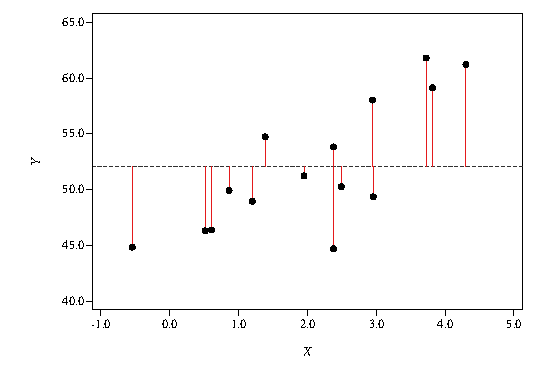
\includegraphics[width=.32\textwidth]{images/hibbs2a.pdf}
  	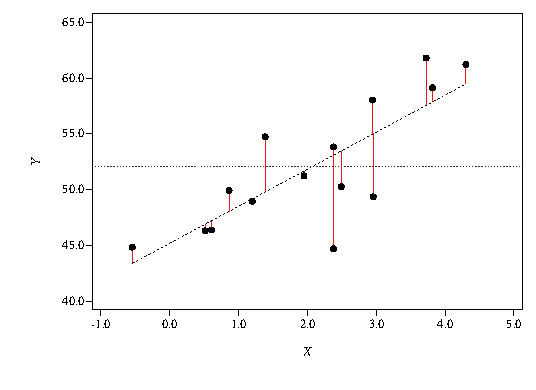
\includegraphics[width=.32\textwidth]{images/hibbs2b.pdf}
  	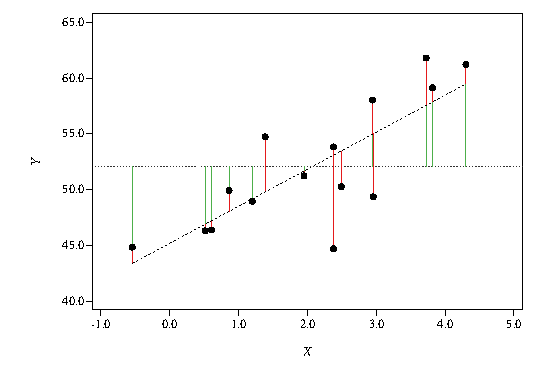
\includegraphics[width=.32\textwidth]{images/hibbs2c.pdf}

  	\caption[Linear fit of U.S. presidential elections]{\label{fig:hibbs_fit}%
  	Linear fit of U.S. presidential elections. %
  	\hibbs}
  \end{figure}%

  Since the null estimator is a sort of parabola for the actual values of the data, linear regression considers that the most effective model will leave as little residuals as possible, hence minimizing $\epsilon$. Since the estimator is of the form $Y = \alpha + \beta X + \epsilon$, the formula for the residuals is $\epsilon = Y_i - \alpha - \beta X_i$. Squaring the error term suppresses the issue of positive and negative values, and their sum, the \emph{residual sum of squares} (RSS), is thus derived from this formula:

  $$\text{RSS} = \sum{\hat{\epsilon}_i^2} = \sum{(Y_i-\hat{\alpha}-\hat{\beta} X_i)^2} \quad (i = 1, \ldots, n)$$

  Minimizing the RSS is at the heart of linear \emph{least squares} estimation, and its empirical success with your data is referred to as the \emph{goodness of fit} of the model. Statistical accuracy is also measured in the minimization of the \emph{root-mean square error} (\label{rmse}RMSE) of the model, explained at p.~\pageref{rmse_explained}. Both measures are statistical and are substantively important only if you can justify so: your research design must aim at predicting as much variance as possible in the overall sample for the goodness of fit of your model to be relevant.

  The actual derivation of least squares estimates, which involves differentiating the parameters $\alpha$ and $\beta$, takes only a few equations to write down but becomes computationally intensive for more than one independent variable. Stata takes all computational aspects in charge for you, and linear regression is virtually always computationally possible with social science data.
  
  \paragraph{Regression output}

  In regression output, the linear estimator for the intercept of the regression line, $\alpha$, is called the \emph{constant}, while the estimated $\beta$ parameters that apply to the independent variable(s) are called regression \emph{coefficients}. Stata performs the parametric estimation of regression coefficients with the \cmd{reg}{regress} command, and can store its results with the \cmd{predict} command.

  \paragraph{Standard output}%
  Table~\ref{tbl:hibbs_yx1_regress} shows the standard output for linear regression in Stata:

  \index{Linear regression!Stata output}%
  \begin{table}[htp]
      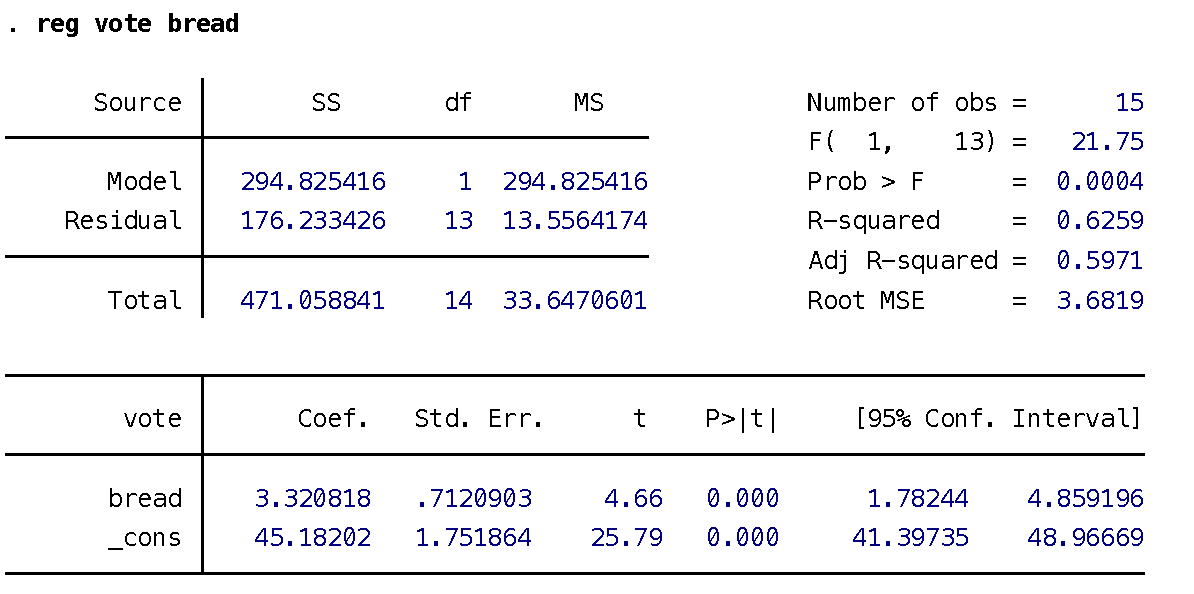
\includegraphics[scale=.5]{images/hibbs_yx1_regress.pdf}

    	\caption[Regression output for a simple linear model]{\label{tbl:hibbs_yx1_regress}%
  	Regression output for a simple linear model. %
  	\hibbs}
  \end{table}%

  % The output is organized in three tables. The \emph{analysis of variance} (top-left) shows how much variance was predicted by the model, and how much is left in the residuals. This information is elaborated in the \emph{goodness of fit} (top-right) of the model. Finally, the \emph{coefficient estimates} (bottom) mention the coefficient for variable $X$ and for the constant (\texttt{\_cons}).

  % %
  % %
  % \subsection{Exercise}
  % %
  % %
  % 
  % \begin{frame}{Exercise}
  % 
  %     \begin{exampleblock}{Ex~8.1. Quality of Government 2011}
  % 
  %       \begin{itemize}
  %         \item Variables: \texttt{d wdi\_gdpc wdi\_mege wdi\_pb2 wdi\_the}
  %         \item Plot correlations and estimate simple linear regressions.
  %       \end{itemize}
  % 
  %     \end{exampleblock}
  % 
  % 
  %   \begin{exampleblock}{Ex~8.2. Quality of Government 2011}
  %       
  %       \begin{itemize}
  %         \item Variables: \texttt{d wdi\_pb2 gol\_polreg }
  %         \item Plot correlations and estimate simple linear regressions, using \texttt{wdi\_pb2}
  %       \end{itemize}
  %       
  %   \end{exampleblock}
  % 
  % 
  % \end{frame}
  % %
  % %  
